\section*{\underline{PART B: Understanding the Response Variable}}
\markboth{PART B: Understanding the Response Variable}{}

\subsection*{Question 4: What does the distribution of machine repair time look like?}

To understand the distribution of machine repair times, we first calculated the descriptive statistics for the dataset. The summary of these metrics is presented in Table\ref{tab:desc_stats}. 

\begin{table}[H]
    \centering
    \begin{tabular}{ll}
        \toprule
        \textbf{Statistic} & \textbf{Value} \\
        \midrule
        Mean & 16.36 minutes \\
        Median & 11.00 minutes \\
        Variance & 492.24 \\
        Standard Deviation & 22.19 minutes \\
        Range & 273.70 minutes \\
        Skewness & 5.60 \\
        Kurtosis & 45.72 \\
        \bottomrule
    \end{tabular}
    \caption{Descriptive Statistics of Machine Repair Time}
    \label{tab:desc_stats}
\end{table}

The mean (16.36 minutes) is notably higher than the median (11.00 minutes), which, along with the high positive skewness (5.60) and heavy kurtosis (45.72), indicates a heavily right-skewed distribution. The large range (273.70 minutes) and high variance highlight the presence of unusually large observations (extended repair times) that pull the mean upward.

To visualize this skewness, we plotted the frequency distribution. Figures \ref{fig:freq1} shows the histogram of repair times bounded between 0 and 100 minutes alongside the log-transformed distribution, which helps visualize the data spread more clearly.

\begin{figure}[H]
    \centering
    \begin{minipage}{0.48\textwidth}
        \centering
        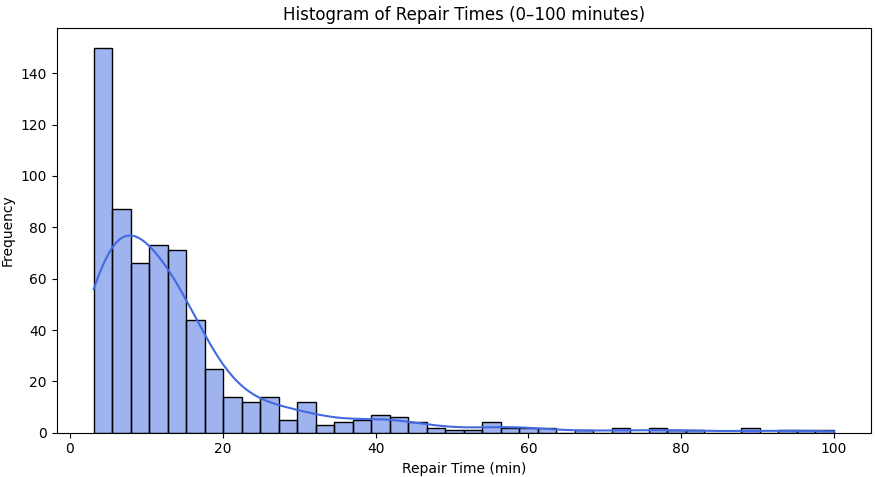
\includegraphics[width=\linewidth]{figures/freq1.png}
        \caption{Histogram of Repair Times (0--100 min)}
        \label{fig:freq1}
    \end{minipage}\hfill
    \begin{minipage}{0.48\textwidth}
        \centering
        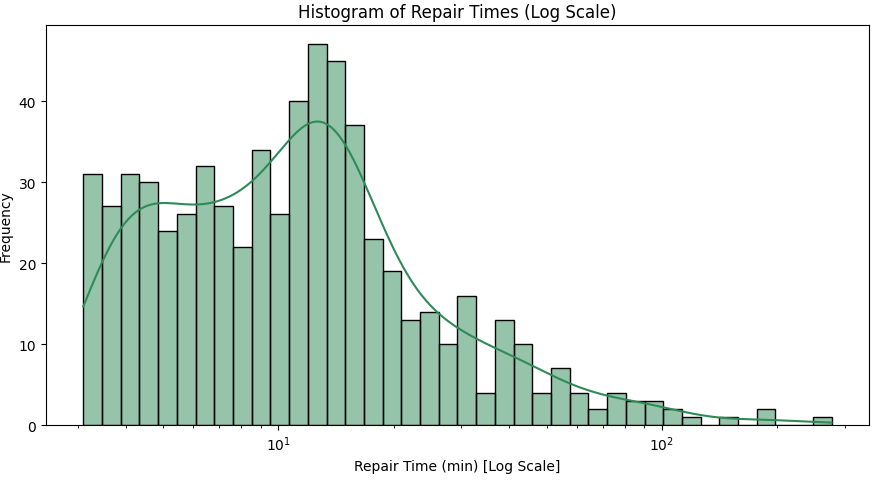
\includegraphics[width=\linewidth]{figures/freq2.png}
        \caption{Histogram of Repair Times (Log Scale)}
        \label{fig:freq2}
    \end{minipage}
\end{figure}

\subsection*{Question 5: Which probability distribution might reasonably represent repair time?}

Given the strictly positive nature of the data and its heavy right-skewed tail (as visualized in Figures \ref{fig:freq1} and \ref{fig:freq2}), the \textbf{Lognormal Distribution} provides a highly reasonable fit for representing machine repair times. 

The estimated parameters for our fitted Lognormal distribution model are:
\begin{itemize}
    \item \textbf{Shape ($\sigma$):} 0.8108
    \item \textbf{Location ($\mu$):} 0.0000
    \item \textbf{Scale:} 10.9702
\end{itemize}

\subsection*{Question 6: Can we estimate useful probabilities about repair time using an appropriate probability model?}

Using the parameters from our fitted probability model, we can estimate specific cumulative probabilities regarding machine downtime to evaluate the company's targets:

% \begin{itemize}
%     \item \textbf{Probability that a repair takes more than 60 minutes:} 0.0181 (1.81\%)
%     \item \textbf{Probability that a repair is completed within 30 minutes:} 0.8926 (89.26\%)
% \end{itemize}

To provide a granular view of the repair time distribution intervals across the entire sample, we calculated the decile breakdown of repair times, summarized in Table \ref{tab:deciles}.




\begin{table}[H]
    \centering
    \begin{tabular}{ccc}
        \toprule
        \textbf{Repair Time Interval (min)} &
        \textbf{Interval Range (min)} &
        \textbf{Cumulative Proportion (\%)} \\
        \midrule
        0.00 -- 3.88   & 3.88  & 10 (0--10) \\
        3.88 -- 5.54   & 1.66  & 10 (10--20) \\
        5.54 -- 7.17   & 1.63  & 10 (20--30) \\
        7.17 -- 8.93   & 1.76  & 10 (30--40) \\
        8.93 -- 10.97  & 2.04  & 10 (40--50) \\
        10.97 -- 13.47 & 2.50  & 10 (50--60) \\
        13.47 -- 16.78 & 3.31  & 10 (60--70) \\
        16.78 -- 21.71 & 4.93  & 10 (70--80) \\
        21.71 -- 31.01 & 9.30  & 10 (80--90) \\
        $> 31.01$      & --    & 10 (90--100) \\
        \bottomrule
    \end{tabular}
    \caption{Repair Time Distribution (Deciles)}
    \label{tab:deciles}
\end{table}

